\subsection{Circuit}

	\subsubsection{Structure}

		Le circuit sera principalement composé de medium de 5mm d'épaisseur (matériau résistant, léger, peu fragile, facilement usinable et peu cher) reposant sur une structure une taseaux (de manière à surelever le plateau, afin de passer les câbles en dessous et laisser de la place pour les systèmes de fixation, par exemple ainsi que pour rigidifier la structure (le medium étant un matériau souple)).\\

		Nous avons décidé de donner à la "piste" du circuit la forme suivante :

		\illu{formePiste.pdf}{Forme de la "piste"  du circuit}{0.6}

		Ainsi, nous avons un carrefour à feux ainsi que quatre intersections, soit un large éventail de possibilités.\\

		Après avoir fait une rapide estimation des dimensions de notre robot, nous avons déduit que le circuit devrait faire environ deux mètres par deux mètres.
		Nous avons préféré ajouter vingt centimètres de côté par sécurité.\\

		Ces dimensions étant importantes, ceci nous a conforté dans l'idée que notre circuit devrait être fait en deux parties afin d'en faciliter le rangement. Nous fabriquerions donc deux cadres de deux mètres vingt par un mètre dix qui pourront être facilement assemblés.

	\subsubsection{Feux}

		Les feux seront comprendront chacun deux LED "haute luminosité" de 5mm : une rouge et une verte. Trois fils seront donc nécéssaires pour chaque feu : deux pour les alimentations de chacune des LEDs et une masse commune. Avec les quatre feux, le circuit comptera donc huit LEDs et douze fils différents.\\
		\newpage
		Les feux seront dans la mesure du possible imprimés en 3D :\\
		\begin{figure}[ht!]
			\centering
			\begin{minipage}{0.4\textwidth}
				\raggedleft
				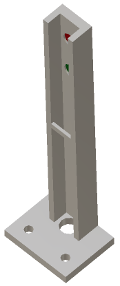
\includegraphics[scale=0.9]{Graphics/feu2.png}
			\end{minipage}\hfill
			\begin{minipage}{0.4\textwidth}
				\raggedright
				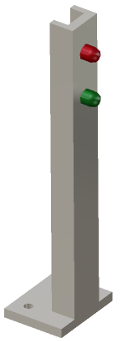
\includegraphics[scale=0.8]{Graphics/feu1.png}
			\end{minipage}
			\caption{Maquette numérique d'un feu bicolore}
		\end{figure}

		\vspace{15pt}

		Notons la présence de deux petits trous pour enficher les feux sur des vis et d'un plus gros pour le passage des fils. Un passe-câble est également intégré à la "goulotte" qui constitue le montant du feu afin de guider les fils.

	\subsubsection{Capteurs}

		Afin d'adapter le comportement des feux à l'état du trafic, encore faut-il que la carte FPGA dispose d'un moyen d'évaluer ce trafic.\\

		Nous disposerons donc sur la piste des capteurs "ILS" (Interrupteur à Lame Souple) \nomenclature{ILS}{Interrupteur à Lame Souple} sur la piste aux abords des feux. Les ILS sont de petits composants se comportant comme un interrupteur ouvert en temps normal, et comme un interrupteur fermé lorsqu'on approche un aimant.\\

		En munissant nos robots d'un aimant bien placé, ces derniers fermeront temporairement le circuit lors de leur arrivée aux abords des feux.\\

		Cette solution est extremement simple et ne nécéssite aucun traitement du signal (contrairement aux capteurs à effet hall ou fourches optiques, souvent utilisés en détection de présence).

\newpage
\subsection{Robot}

	\subsubsection{Suivi de trajectoire}

		Afin d’offrir une capacité de suivi de trajectoire simple et robuste, il a été décidé d’intégrer au robot la fonctionnalité "suivi de ligne". Il s’agit de l’une des méthodes les plus répandues\cite{bib3} \cite{bib4}, relativement simple à implémenter et économe aussi bien en composants qu’en puissance de calcul nécessaire.\\

		L’idée est d’offrir une base fiable et simple pour que le suivi de trajectoire ne soit pas une source de préoccupation ou d’erreur dans le cas d'utilisations centrées sur d’autres problématiques (dans le cadre d'un TP sur la reconnaissance d'image, par exemple). Cela n’exclut cependant pas qu’un étudiant ou chercheur désireux d’explorer d’autres possibilités de suivi de trajectoire (via la caméra, un dispositif de triangulation ou autre) puisse se passer de ce module et exploiter une autre solution.\\

		Le principe de suivi de ligne est relativement simple : on place sur l’axe du robot, quelques millimètres au-dessus du sol, un capteur appelé « réflecteur optique ». Ce capteur émet une onde lumineuse (souvent infrarouge) et une cellule mesure l’intensité reçue sur la longueur d’onde émise. Une forte intensité reçue indiquera la présence d’une surface réfléchissante, tandis qu’une faible intensité indiquera la présence d’une surface absorbante. Il est ainsi aisé de différencier un fond sombre (la « route ») d’une ligne blanche.\\

		Une loi linéaire lie la tension lue en sortie de capteur à l'intensité reçue.\\
		Une simple lecture de cette tension permet, après comparaison avec des valeurs "seuil" définies expérimentalement, de savoir si le capteur se trouve au dessus d'une ligne blanche ou non.\\

		Sur les schémas suivants, pour des raisons d'imprimabilité et de lisibilité, les lignes seront noires et le revêtement du circuit sera blanc.\\

		\begin{figure}[H]
			\centering
			\begin{minipage}{0.48\textwidth}
				\centering
				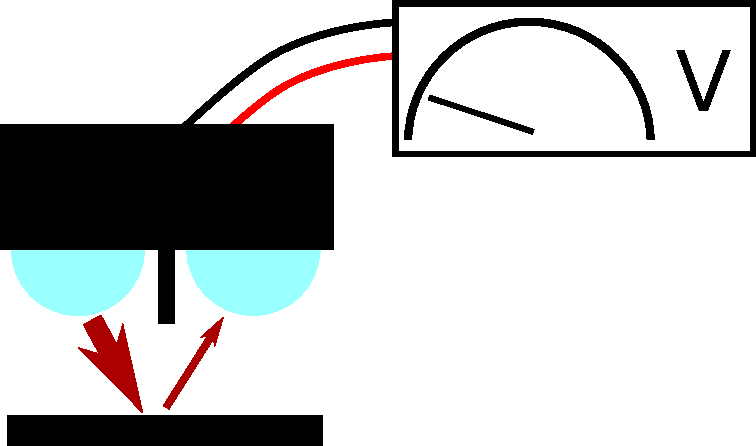
\includegraphics[scale=0.45]{Graphics/capteurOptiqueFondNoir.pdf}
				\caption{Capteur au dessus d'un support sombre}
			\end{minipage}\hfill
			\begin{minipage}{0.48\textwidth}
				\centering
				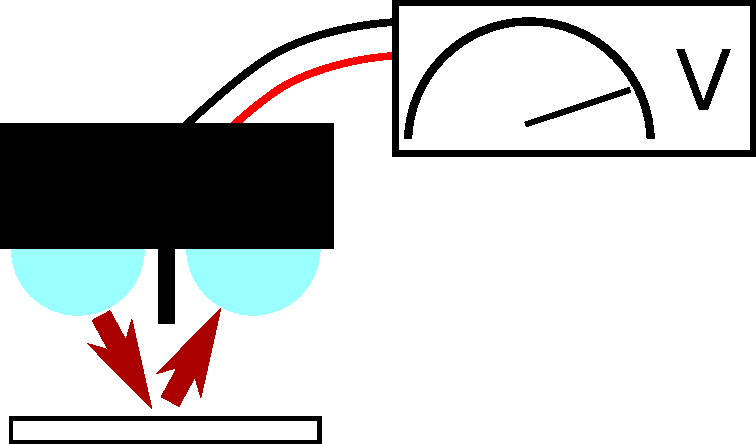
\includegraphics[scale=0.45]{Graphics/capteurOptiqueFondBlanc.pdf}
				\caption{Capteur au dessus d'un support clair}
			\end{minipage}
		\end{figure}

		La question qui se pose est celle du nombre de capteurs, et de leur disposition.\\

		Il est tout à fait possible de n'utiliser qu'un capteur : chaque fois qu'il quitte la ligne blanche, on entamera un virage à droite (puis à gauche si on ne retrouve pas la ligne blanche dans les quelques millisecondes suivantes) jusqu'à retrouver la ligne. Il est évident que cette méthode ne permettra pas une très grande fluidité de déplacement pour notre robot.

		\illu{capteurSimpleGauche.pdf}{Dépassement de la ligne sur la gauche}{1}
		\illu{capteurSimpleDroite.pdf}{Dépassement de la ligne sur la droite}{1}

		L'utilisation de deux capteurs permet une meilleure fluidité. On placera cette fois un capteur de chaque côté de la ligne.

		\illu{capteurDoubleGauche.pdf}{Dépassement de la ligne sur la gauche}{1.4}
		\illu{capteurDoubleDroit.pdf}{Dépassement de la ligne sur la droite}{1.4}

		Notons que, quelque soit la méthode employée, le suivi de ligne se résume toujours à un "rebondissement" des capteurs sur la ligne. Aussi, pour obtenir une trajectoire aussi rectiligne que possible, il faudra "resserer" les capteurs au maximum autour de la ligne, et appliquer des corrections de faible amplitude.

		\illu{capteurDoubleEcartFort.pdf}{Ecart important entre les capteurs}{1}
		\illu{capteurDoubleEcartFaible.pdf}{Ecart réduit entre les capteurs}{1}

		Nous pourrons éventuellement introduire un amortissement progressif de la correction via un régulateur PID\nomenclature{PID}{Proportionnel, Intégrateur, Dérivateur}, mais cela peut introduire de nombreuses problématiques dans des cas d'utilisation plus complexes.\\

		Nous retiendrons donc à ce stade la solution consistant en deux capteurs placés de part et d'autre de la ligne. Nous veillerons à ce que le placement des capteurs permette une détection de très faibles écarts de trajectoire, sans pour autant induire des ambiguïtés de mesure.\\

		Intéressons nous maintenant au cas d'une trajectoire courbe. Le fait d'avoir privilégié l'application de faibles corrections peut alors s'avérer problématique si ces dernières ne sont pas suffisantes pour adapter la trajectoire.

		\illu{perteTrajectoireVirage.pdf}{Perte de trajectoire en virage dû à de trop faibles corrections}{1.5}

		Pour obtenir un fluidité de déplacement raisonnable tout en assurant la possibilité de suivre des trajectoires courbes à rayon de virage réaliste, nous placerons une deuxième série de capteurs "encadrant" les capteurs principaux. Une détection de ligne par ces capteurs déclanchera une correction plus importante.

		\illu{trajectoireVirage.pdf}{Maîtrise de la trajectoire en virage grâce à l'utilisation de 4 capteurs}{1.5}

		Cette solution consistant en l'utilisation de quatre réflecteurs optiques alignés de manière à encadrer de près la ligne à suivre est sans doute l'une des plus simples imaginables en terme de réalisation mais également d'utilisation et de maintenance.
		Elle n'est malheureusement pas suffisante pour répondre à notre besoin. En effet, cette solution trouvera ses limites dès lors que notre Robot rencontrera sa première intersection, élément capital de ce projet.\\

		\illu{intersection4Capteurs.pdf}{Robot incapable de répondre à la présence d'une intersection}{1.5}

		Si on trouve dans la littérature de très nombreux exemples de réalisations de robots suiveurs de lignes, ces dernières se limitent toujours à des circuits sous forme de boucle. Notre défi est donc de mettre au point une solution permettant l'évolution du robot sur un circuit comprenant des intersections. Notre robot devra ne pas être "perturbé" au passage d'une intersection, mais surtout être capable d'emprunter toutes les directions qui lui sont offertes.\\

		La solution que nous avons mis au point consiste en l'introduction d'un capteur central et l'adoption d'un comportement "mono-latéralement centré" du robot lors de la traversée d'intersections : lorsqu'il arrivera sur une intersection, le robot ne se souciera plus que de garder son capteur central sur la ligne, et ses capteurs latéraux \textbf{du côté de la direction choisie} à l'écart de cette dernière.

		\illu{intersection5CapteursTD.pdf}{Suivi de trajectoire sur une intersection (en choisissant d'aller tout droit)}{1.5}
		\illu{intersection5CapteursDroite.pdf}{Suivi de trajectoire sur une intersection (en choisissant d'aller à droite)}{1.5}

		Notons que la forme de la ligne devra être intelligemment faite, en présentant des rayons de courbure réalistes (un véhicule ne peut pas tourner à angle droit) et des intersections réalisables (notamment via l'utilisation de deux lignes séparées pour la circulation en sens contraires).\\

		Voici donc à quoi ressemblerait un carrefour:
		\illu{carrefour.pdf}{Carrefour en représentation "lignes"}{1.4}

		Pour pleinement définir la logique mise au point, illustrons la au travers de la situation la plus complexe que pourra rencontrer notre robot, qui est celle de la bifurcation à gauche.

		\illu{carrefour5capteursGauche.pdf}{Cas du virage à gauche sur un carrefour avec cinq capteurs}{1.5}

		\begin{enumerate}
			\item Le premier croisement ne nous intéresse pas. Nous allons continuer tout droit et éteignons donc la moitié droite de nos capteurs.
			\item Au passage du croisement, nous éteignons temporairement l'ensemble de nos capteurs.
			\item Le croisement passé, nous éteignons cette fois la moitié gauche de nos capteurs pour ne pas être perturbés par "la voie d'insertion".
			\item Peu de temps après, nous rallumons la moitié gauche et éteignons la moitié droite des capteurs pour suivre la voie bifurquant à gauche.
		\end{enumerate}

		Cette solution semble robuste tout en conservant une certaine simplicité d’implémentation. Elle sous-entend en revanche que le robot "sache" quand il arrive sur une intersection, mais également qu'il puisse évaluer à quelques millimètres près la distance qui le sépare des différentes "parties" de cette intersection (pour activer et désactiver ses capteurs en conséquence).\\

		La solution à cette problématique nous a été inspirée par le souvenir d'un brevet déposé en 2003 par le groupe PSA \cite{bib5}, qui proposait l'utilisation de code-barres tracés sur la route et que des capteurs placés sous le pare-choc des voitures pourraient "lire" pour prévenir le conducteur des sources de danger à venir (intersections, feux...).
		Il fut donc décidé que deux capteurs supplémentaires seraient ajoutés sur les extérieurs. Ils augmenteraient ainsi la précision de placement sur la ligne, mais permettraient surtout de lire des "codes-barres" placés sur la piste. Ces code-barres devraient permettre au robot d'être averti de l'approche d'un carrefour (trois choix de direction possibles) ou d'une simple intersection (deux choix possibles). Nous avons simplement basé notre code sur une ligne simple ou doublée :\\
		\begin{figure}[H]
			\begin{tabu}to \textwidth {@{} | l | *3{X[c]|}@{}}
			  \hline
			   & \textbf{Gauche} & \textbf{Droite} & \textbf{Gauche ET Droite} \\
			  \hline
			  \textbf{Simple} & Impossible de tourner à droite & Impossible de tourner à gauche & Toutes possibilités offertes\\
			  \hline
			  \textbf{Double} & Obligation de tourner à gauche & Obligation de tourner à droite & Impossible d'aller tout droit \\
			  \hline
			\end{tabu}
			\caption{Formalisme employé pour les code-barres}
		\end{figure}

		Un code "doublé" serait composé de deux lignes elles mêmes séparées d'une épaisseur de ligne.
		Les codes seraient placés à 30cm du premier croisement.\\

		Dès la lecture d'un code au sol, le robot sera donc "attentif" à l'éventuelle apparition d'un doublon pendant environ deux centimètres. Si rien n'est lu passé cette distance, il en déduira qu'il s'agit d'un code simple. Il prendra alors une décision de direction (et pourra au passage en avertir les autres robots) et commencera un décompte de distance afin de gérer les activations et désactivations de ses capteurs jusqu'au franchissement de l'intersection.\\


		Illustrons ce système avec le cas de la bifurcation à gauche :

		\illu{carrefour7capteursGauche.pdf}{Cas du virage à gauche sur un carrefour avec sept capteurs}{1.5}

		\begin{enumerate}
			\item Lecture d'un code-barre : dans 30cm le robot aura la possibilité de tourner à droite et à gauche.
			\item Aucun doublon détecté dans les quelques centimètres suivants. La possibilité d'aller tout droit nous est donc offerte. Prise de décision quant à la direction (nous choisissons d'aller à gauche) et avertissement des autres robots en conséquence.
			\item Le premier croisement ne nous intéresse pas. Nous allons continuer tout droit et éteignons donc la moitié droite de nos capteurs.
			\item Au passage du croisement, nous éteignons temporairement l'ensemble de nos capteurs.
			\item Le croisement passé, nous éteignons cette fois la moitié gauche de nos capteurs pour ne pas être perturbés par "la voie d'insertion".
			\item Peu de temps après, nous rallumons la moitié gauche et éteignons la moitié droite des capteurs pour suivre la voie bifurquant à gauche.
		\end{enumerate}

		Le robot doit donc être conscient des distances parcourues avec une précision supérieure à deux centimètres. Le moyen le plus simple d'implémenter cette fonctionnalité est sans aucun doute au travers d'un encodeur incrémental placé sur l'axe de propulsion du robot.\\

		Nous pouvons donc considérer qu'à ce stade, nous disposons d'un solution satisfaisante répondant à la problématique du suivi de trajectoire.
		Cette solution répond précisément aux contraintes du projet, tout en conservant un certain niveau de simplicité. Elle est, pour rappel, constituée des éléments suivants :\\

		\begin{itemize}
			\item \textbf{Sur le circuit :} Un réseau de lignes blanches sur fond noir représentant les trajectoires empruntables par le robot.
			\item \textbf{Sur le robot :} Un ensemble de 7 réflecteurs optiques.
		\end{itemize}

	\subsubsection{Détection d'obstacles et de de signalisation}

		Etant donné le fait que les robots évoluerons dans un environnement idéal, parfait, il n'existera pas en première instance d'obstacles à proprement parler, tel qu'une route barrée aléatoirement, par exemple. Le seul obstacle que nous risquerions de rencontrer est un autre robot situé juste devant nous et arrété à un feu. Ici, le sonar situé à l'avant aura une priorité plus élevée que les autres capteurs, et pourra passer outre les différentes informations reçus par les autres capteurs, influençant fortement la décision. En langage informatique, on parlera d' "override", qui peut être nécessaire dans une situation d'urgence comme celle ci. Ainsi, quelque soit les informations des autres capteurs, le robot s'arretera.
		\\
		Ce point est bien entendu sujet à améliorations, et tout développeur pourra, s'il le désire, implémenter la gestion de ce genre de situations : route barrée, ligne centrale partiellement effacée et peu détectable, etc...
		\\\\
		Dans le cadre de ce projet, cette détection de signalisation se limite aux feux et aux intentions des vehicules comme nous allons le developper en \ref{feuEtIntentions}, page \pageref{feuEtIntentions}. Cependant, il pourra être envisageable à l'avenir de rajouter une signalisation par panneaux (Céder le passage, Stop...).
		Cette partie sera réalisée en utilisant des techniques de reconnaissance d'image en quasi-temps réel, utilisant la caméra embarquée, et initialement développé en Python.
		\\\\
		Notons également qu'une série des tests simples et logiques seront réalisés en cascade. Une fois tous ces tests (détaillés ci-dessous) effectués, le module de décision du robot réalisera une synthèse de tous les résultats, et effectuera un choix.
		\begin{enumerate}
			\item Attente de lecture du premier code-barre
			\item Lecture du premier code-barre
			\item Démarrage du décompte de la distance
			\item Attente de lecture du deuxième code-barre
			\item S'il existe, lecture
			\item Décision sur la direction à prendre
			\item Signalisation des intentions
			\item Recherche du feu de signalisation
			\begin{enumerate}
				\item S'il existe, détermination de sa couleur
				\begin{itemize}
					\item Arrêt à 10 cm s'il est rouge
					\item S'il est vert, on continue
				\end{itemize}
				\item S'il n'existe pas, on se situe à une intersection "classique", recherche d'un robot éventuel
				\begin{itemize}
					\item S'il y a un robot, sommes-nous prioritaire ? Est-il déjà engagé ? On utilisera, en plus de la reconnaissance d'image, le sonar.
					\item S'il n'y en a pas, on continue sans s'inquiéter.
				\end{itemize}
			\end{enumerate}
			\item Une fois que le carrefour ou l'intersection est passé, on éteint toute indication sur nos intentions.
		\end{enumerate}
		Une fois cette séquence terminée, on recommence.
		\\
		En parallèle, une instance vérifiera en boucle si un obstacle se situe devant nous. Si oui, le système d' "override" s'applique. Nous nous arretons et mettons en pause la tâche en cours jusqu'à ce que l'avancée soit possible, plus un délai de sécurité. Le robot pourra se remettre en mouvement et reprendre la tâche mise en pause.


	\subsubsection{Implémentation matérielle}

		\paragraph{Propulsion et direction}

			D’expérience, nous avons constaté que quatre roues complexifient et sur-contraignent les manœuvres directionnelles des robots. Nous avons donc décidé d'adopter la solution la plus répandue en "petite robotique" et consistant en l'utilisation de deux moteurs à courant continu pilotés indépendamment assurant à la fois la propulsion et la direction : on réduira les gaz à droite pour tourner de ce côté et réciproquement. Ces moteurs sont généralement pilotés en "PWM" \nomenclature{PWM}{Pulse-Width Modulation, ou Modulation de Largeur d'Impulsions}, mais d'autres solutions sont possibles et dépendront de notre contrôleur. Beaucoup d'applications utilisent des chenilles ou des courroies en caoutchouc pour assurer la propulsion, mais nous privilégierons l’utilisation de roues à pneus, par soucis de simplification de la conception (l'emploi de chenilles ou de courroies induit  une grande précision d'usinage et de montage pour assurer le parallélisme des poulies et la tension de la courroie) et de réduction des coûts.\\

			L'utilisation d'un seul moteur de propulsion et d'une roue directionnelle pilotée par un servomoteur a longtemps été considérée, mais cette solution s'est révélée bien plus complexe à mettre en place et sans réel intérêt particulier.\\

			\illu{virageDeuxMoteurs.pdf}{Virage à l'aide de deux moteurs indépendants}{1.5}

			L'espacement entre les deux roues $E$ est constant et connu.
			On fixera la vitesse appliquée à la roue à l'extérieur du virage $\omega_{ext}$ comme référence.
			On adaptera donc la vitesse de la roue à l'intérieur du virage $\omega_{int}$ en fonction du rayon de virage $R$ désiré.
			Il s'agit là d'une simple relation de Thales et on définit ainsi :
			\[\omega_{int} = \omega_{ext}\frac{R-E}{R}\]

			On peut donc obtenir n'importe quel rayon de virage en diminuant simplement la vitesse de la roue à l'intérieur du virage.
			L'approximation selon laquelle la tension appliquée à un moteur et sa vitesse de rotation sont linéairement liés sera amplement suffisante dans le cadre de ce projet.\\

		\paragraph{Controleur}\label{Solution-controleur}

			Nous cherchons un contrôleur capable d'embarquer des applications en C (ou ses dérivés) et si possible en Python et/ou Matlab.
			Ce contrôleur devra être capable d'acquérir les données de différents capteurs et de commander deux moteurs au minimum (sans compter d'éventuelles sorties type LEDs).
			Le contrôleur devra également bénéficier d'une puissance de calcul suffisante pour les opérations de reconnaissance d'image.\\

			Ce dernier critère élimine d'office les microcontrôleurs 8 et 16 bits et donc les cartes de type "Arduino" dont la puissance de calcul et la capacité de traitement de flux est bien trop faible pour permettre une reconnaissance d'image supérieure à quelques pixels carrés.\\

			Nous nous sommes naturellement tournés vers la famille des micro-ordinateurs mono cartes. Cette récente catégorie d'ordinateurs propose sur une carte de quelques centimètres de côté et pour moins d'une centaine d'euros un véritable ordinateur avec une connectivité réseau et USB, bien souvent vidéo, une puissance de calcul extrêmement confortable et la capacité de faire tourner des systèmes Linux et dérivés (et donc d’exécuter tous types de codes). Démocratisés en 2011 avec le Raspberry-Pi, ces ordinateurs se sont multipliés et l'offre est aujourd'hui très large. Nous avons ciblé notre sélection sur les plus rependus (qui sont, de par leur succès, bien plus abordables et faciles à se procurer, et bénéficient d'une plus large et solide base documentaire) : les Raspberry-Pis, Beaglebones et UDOOs (pour ne citer qu'eux).\\

			Les UDOOs furent vite écartés en raison de leur prix.
			Le Raspberry-Pi 2 et BeagleBone Green se situent dans la même gamme de prix (autour de 40\$). Nous avons arrêté notre choix sur le BeagleBone Green (BBG\nomenclature{BBG}{BeagleBone Green}): ce dernier, contrairement au Raspberry-Pi 2, ne dispose pas de sortie vidéo (dont nous n'avons pas utilité au sein de ce projet) et possède une puissance de calcul légèrement inférieur à ce dernier (tout en restant parfaitement respectable) mais possède une mémoire intégrée (ce qui dispense de l'achat d'une carte séparée) et surtout de capacités d'entrées/sorties numériques et analogiques bien supérieures. Ce point nous est extrêmement important: en effet, le Raspberry-Pi n'est capable de générer qu'un signal PWM et ne possède aucune entrée analogique ce qui aurait nécessité l'utilisation de "périphériques" supplémentaires pour la gestion des moteurs et des capteur et donc alourdi les coûts et la complexité de conception, augmenté le nombre de sources potentielles de pannes...\\

			Nous utiliserons donc un BeagleBone-Green Wireless :
			\illu{BBG.jpg}{Le BeagleBone Green \textit{\textbf{(source : seeedstudio.com)}}}{0.45}

			Ce dernier est équipé d'un processeur ARM 32bits à 1Ghz, de 512Mo de RAM de 4Go de mémoire embarquée et d'un impressionnante capacité de communication : 7 entrées analogiques (la carte comprend un convertisseur analogique-numérique 12bits), 65 entrées/sorties numériques (0 ou 3.3V) et bénéficie même de fonctionnalités telles qu'un compteur d'impulsion intégré au processeur (particulièrement utile pour l'interfaçage de notre encodeur). La connectivité wifi et bluetooth offre de belles possibilités quant aux interfaces utilisateur et la capacité de communiquer entre robots. La carte consomme moins de 1,5W et coûte 45\$ \cite{bib6}.
			Nous la "chapeauterons" d'une carte d'extension que nous réaliserons nous même pour faire l'interface entre les ports d'extension et nos différents capteurs et actionneurs (voir \ref{carteMere}, page \pageref{carteMere}).\\

			Notons que le BBG doit être alimenté en 5V, et travaille avec un niveau logique "CMOS" de 3.3V. Les entrées et sorties numériques devront donc être compatibles (niveau haut supérieur à 2.5V et inférieur ou égal à 3.3V et niveau bas inférieur à 1.3V).

		\paragraph{Suivi de ligne}\label{solutionSuiviLigne}

			Comme dit précédemment, nous utiliserons sept réflecteurs optiques infrarouges pour effectuer le suivi de ligne.
			Un réflecteur optique est composé d'une LED \nomenclature{LED}{Light-Emitting Diode, ou Diode Electro-Luminescente} (ici infrarouge) et d'un phototransistor. Le phototransistor est comparable à un transistor classique, dont le courant de base serait remplacé par une intensité lumineuse, ou plus simplement encore comme une résistance variable en fonction de l'intensité lumineuse reçue.\\

			Nous utiliserons des TCRT5000, très répandus.\\

			Les capteurs nous fournissent donc une tension variable qu'il faudra pouvoir exploiter : en dessous d'une certaine valeur de cette tension, nous pourrons conclure en la présence d'une ligne blanche (forte réflectivité).\\

			Deux solution s'offrent à nous : ou bien concevoir un montage basé sur un comparateur et une résistance variable (pour régler la valeur seuil) afin d'obtenir une sortie booléenne (par exemple : 5V en présence d'une ligne blanche et 0V sinon) qui pourra très simplement être lue sur n'importe quelle entrée numérique du contrôleur, ou bien tirer partie de l'encodeur analogique-numérique intégré au contrôleur pour lire la valeur directement. Nous privilégierons cette méthode qui permet de limiter le nombre de composants, et donc le coût et les sources de pannes.\\

			Le BeagleBone Green possède sept entrées analogiques (nous avons justement sept capteurs) capables de discerner $2^{12} = 4096$ niveaux différents linéairement répartis entre 0 et 1,8V\cite{bib6}.
			Ainsi, l'application d'une tension de 0V à l'une de ce entrées nous permettra de lire la valeur "0" logiciellement, 2048 pour 0,9V, 4096 pour 1,8V etc... Nous prendrons garde à ne jamais dépasser cette valeur sous peine d’endommager le controleur. Le BBG fournit une tension de 1.8V spécifiquement pour cette application\cite{bib6}.\\

			L'intégration des capteurs est discutée en \ref{integrationReflecteurs} (page \pageref{integrationReflecteurs}).

		\paragraph{Acquisition d'images}

			L'acquisition d'images, pour des raisons évidentes de coûts et  de simplicité d'utilisation, sera réalisée à l'aide d'une webcam standard de bureau, connectée en USB au BeagleBone. Nous avons donc choisi d'utiliser la Webcam Logitech C170 :
			\illu{Logitechc170.png}{Webcam Logitech C170 \textbf{\textit{(source : Logitech)}}}{0.35}
			Compte tenu du fait que les caractéristiques techniques du BeagleBone ne nous permettait pas de traiter de la Haute Définition en quasi-temps réel, et que nous n'avions pas besoin d'un tel niveau de précision, nous nous sommes donc intéressés à cette caméra qui, en plus d'être d'une qualité acceptable, possède un clip de fixation universel, facilitant ainsi la mise en place sur le robot. \\

			L'acquisition logicielle sera réalisée par un script réalisé en \href{https://www.python.org/}{Python}. Avec l'aide du package \href{https://www.http://opencv.org/}{OpenCV}, il est aisé d'interfacer la caméra ainsi que de paramétrer le flux vidéo (taille de l'image, nombre d'images par seconde...) afin d'alléger la charge de traitement de l'image pour ne pas déteriorer les performances du BBG. Les images ainsi récupérées (~10/s) seront ensuite analysées selon plusieurs critères (couleurs et leur position, contours...) afin de participer à une prise de décision fiable et pertinente.
			
		\paragraph{Évaluation des distances}

			\subparagraph*{Distances parcourues}

				L'évaluation des distances parcourues se fera simplement au travers d'un encodeur incrémental placé sur l'un des deux axes de propulsion du robot. Un encodeur incrémental produit au moyen de capteurs optiques ou magnétiques un signal carré dont chaque période correspond au passage d'un élément de référence devant son capteur.
				Ainsi, si on place une roue comprenant quatre éléments de référence (4 aimants, ou 4 obturateurs) régulièrement espacés sur l'axe d'un moteur et le capteur judicieusement, nous pourrons observer un front montant chaque fois que le moteur effectue un quart de tour. En comptant à la fois les fronts montants et descendants, nous connaîtrons les variations angulaires du moteur avec une précision d'un huitième de tour. Et en plaçant un second capteur en quadrature (en déphasage de 90 degrés), notre précision sera doublée.\\

				Le constructeur de nos motoréducteurs, Pololu, propose dans son catalogue un ensemble compatible avec notre motoréducteur comprenant un encodeur à deux capteurs optiques en quadrature et des roues intégrant une mire optique adaptée.

				\illu{encoder.jpg}{Ensemble motoréducteur, roue et encodeur \textbf{\textit{(source : Pololu)}}}{0.25}

				Cette solution nous garantit une compatibilité directe, et nous évite surtout d'avoir à adapter un encodeur (souvent coûteux) sur l'axe entre la roue et le réducteur. L'utilisation des deux capteurs en double fronts nous offre une résolution de 48 impulsions par tour de roue. La roue ayant un diamètre de 42mm, cela nous donne une précision de lecture de :
				\[\frac{\pi \times 42}{48}=2.75mm\]

				Nous pourrons même nous permettre de n'utiliser qu'un capteur et bénéficier ainsi d'une résolution de 5.5mm, répondant largement à nos critères.\\

				Il s'agira ensuite de compter le nombre de fronts montants et descendants sur le signal généré par le capteur.
				Ceci peut se faire simplement en connectant le capteur à une entrée numérique du contrôleur et en observant les changements d'état de cette entrée, mais cette méthode consomme énormément de ressources pour une tâche aussi simple. Une autre solution, quand le processeur le permet, consiste à demander au processeur de détecter les fronts électroniquement et de déclencher un script (compteur) le cas échéant. Cette solution est évidemment préférable lorsqu'elle est disponible.\\

				Par chance, notre processeur ARM-A8 possède cette fonctionnalité et intègre même un module eQEP\cite{bib12} \label{eQEP}\nomenclature{eQEP}{Enhanced Quadrature Encoder Pulse, ou Pulsation d'Encodeur en Quadrature Améliorée} justement dédié au traitement des signaux d'encodeurs en quadrature et qui fera tout le travail à notre place (pour peu que l'on utilise un noyau Linux compatible avec le driver de ce module).

			\subparagraph*{Distance des obstacles}

				La distance avec les obstacles en avant sera mesurée grâce à un sonar HC-SR04. Ce capteur a l'avantage d'être facilement utilisable et est suffisament précis, compte-tenu de notre besoin. De plus, il est également peu sujet aux interférences.
				\illu{sonar.jpg}{Sonar ultrasons HC-SR04 \textbf{\textit{(source : Instructable)}}}{1}
				Cette fonction sera particulièrement utile afin de s'assurer que le robot ne rentrera pas en collision avec un potentiel robot situé sur sa trajectoire.\\
				
				Le principe de fonctionnement est simple : on mesure le temps $t_{echo} $ séparant une impulsion envoyée ("trigger") et le retour de cette impulsion ("echo"). Un simple calcul nous donne ensuite la distance à l'obstacle : $d_{obstacle} = \frac{t_{echo} \times v_{son}}{2}$, avec $v_{son}$ la vitesse du son égale à $340 m.s^{-1}$, selon les Conditions Normales de Température et de Pression.

		\paragraph{Signalisation de ses intentions}

			Nos robots seraient considérés, en théorie de l'intelligence artificielle, comme des "agents". Ils en possèdent en effet toutes les caractéristiques et notamment celle de l'autonomie. Chaque robot est autonome dans le sens où il prend ses propres décisions sans recevoir de commande extérieure. Il est donc primordial que chaque robot puisse avertir les autres de ses intentions, et lui même décrypter les intentions des autres agents.\\

			Nous pourrions atteindre cet objectif en faisant communiquer les robots via un réseau quelconque, mais cela sous-entendrait que ces derniers ne soient capables d'évoluer qu'au milieu de leurs "congénères", ce qui serait parfaitement irréaliste dans la vraie vie. Nous avons donc décidé d'implémenter de simples clignotants et feux stops à LED, simples à mettre en œuvre et universels.

		\paragraph{Interaction avec l'utilisateur}

			Ayant constaté au cours de travaux pratiques qu'il est souvent peu aisé de gérer le déclenchement des séquences de programmes (obligation de passer par des temporisateurs et de brancher/débrancher l'alimentation de la carte), nous avons décidé d'implanter un simple bouton poussoir (qui pourra servir pour démarrer, mettre en pause ou arrêter un programme, par exemple) ainsi qu'un interrupteur commandant l'alimentation de la carte mère (et donc de l'ensemble du système).

		\paragraph{Batterie}

			Pour rappel, voici la liste des composants qu'il nous faudra alimenter :
			\begin{itemize}
				\item Deux moteurs à courant continu\\
				D'après leur fiche technique\cite{bib8}, ces derniers fonctionnent entre 3 et 9V avec un rendement optimal autour de 6V. Leur consommation "axe bloqué" (en couple maximum) est de 1,6A. Une estimation pessimiste de leur consommation en fonctionnement normal consistant à prendre le quart de ce courant, nous pouvons considérer que chaque moteur consommera en moyenne moins de 400mA.
				\item Un BeagleBone Green\\
				Le BBG doit être alimenté en 5V et a une consommation moyenne de 400mA \cite{bib13}.
				\item Sept capteurs IR\\
				Chaque capteur consommant, en tout, environ 35mA.
				\item Une moyenne (généreuse) de 2 LEDs allumées\\
				Avec une consommation d'environ 20mA par LED.
				\item Divers petits composants\\
				Pour lesquels on fera un devis global pessimiste à 100mA.
			\end{itemize}

			Soit une consommation moyenne extrêmement pessimiste de 1600mA.
			La plus haute tension nécessaire (demandée par les moteurs) est d'environ 6V.\\

			Étant donné qu'il est plus difficile de réduire une tension que de l'augmenter, et un moteur à courant continu étant beaucoup plus souple que le reste des circuits électroniques (le moteur ne souffrira pas de tourner à une tension légèrement inférieure) nous privilégierons l'usage d'une batterie de 6V ou plus et d'une capacité supérieure à 1600mAh.


	\subsubsection{Implémentation logicielle}

		Nous ne rentrerons ici pas dans les détails, d'une part car le but n'est pas de procéder à la partie développement dans ce dossier et d'autre part car la partie logicielle représente la part la plus fluctuante de nos robots, destinés à être reprogrammés tout au long de leur cycle de vie. Cependant, nous allons tenter de détailler rapidement l'approche que nous recommandons au sujet du développement logiciel dans le cadre de ce projet.

		\paragraph{Suivi de ligne}

			Le suivi de ligne, en terme de programmation, est une simple problématique de régulation. Nous recueillerons les données issues des différents capteurs, les traiterons, et produirons une réponse au travers des actionneurs.\\

			La question, au delà de celle des logiques et algorithmes utilisés pour produire cette régulation, ici hors sujet, est celle de l’interaction avec les capteurs et actionneurs.\\

			Nos programmes devront faire l'acquisition des données suivantes :
			\begin{itemize}
				\item Données issues des réflecteurs, sous la forme de la valeur de sept tensions.
				\item Données issues de l'encodeur, sous la forme d'un comptage des pulsations.
			\end{itemize}

			Ils devront communiquer leurs ordres en faisant varier la tension aux bornes des moteurs. Ceci se fera au travers de la création d'un signal "PWM".\\

			Il s'agira donc d'établir le lien entre les interfaces d'entrées/sorties du contrôleur et le code à proprement parler.\\

			Sur le BBG, l'un des moyens les plus simples d'effectuer cela est de passer par la bibliothèque Python crée à cet effet par Justin Cooper \cite{bib14} \cite{bib15}. Cette bibliothèque simplifie grandement ce genre d'opérations, et lire la valeur (numérique ou analogique) d'un port, ou changer cette valeur ne prend que deux lignes de code (se référer à la documentation).\\

			Une utilisation des entrées/sorties reste néanmoins possible et accessible en C et C++, par exemple \cite{bib16}, mais nous favoriserons l'utilisation de Python pour des raisons "d'affinité", mais également car ce langage simplifie l'utilisation de nombreux outils nécessaires à ce projet, notamment la communication réseau et le traitement d'images, et ne nécessite aucune compilation.\\

			Nous veillerons cependant, toujours dans un soucis de modularité, à ce que nos "modules" python, soient compatibles avec d'éventuelles réalisations en C, java ou autre (voir \ref{integrationLogicielle} : Intégration Logicielle, page \pageref{integrationLogicielle}).

		\paragraph{Reconnaissance d'image}\label{feuEtIntentions}
			

			La reconnaissance d'image sera utilisée à plusieurs fins :
			\begin{itemize}
				\item \textbf{Couleur du feu}
					La détection de la couleur du feu est un aspect primordial de ce projet. Grâce au package OpenCV, il est très facile de décomposer le spectre de la lumière visible, et donc de déterminer s'il y a en face de nous une lumière verte ou rouge, comme le montre la figure suivante :
					\begin{figure}[H]
					    \centering
					    \begin{subfigure}[h]{0.5\textwidth}
					        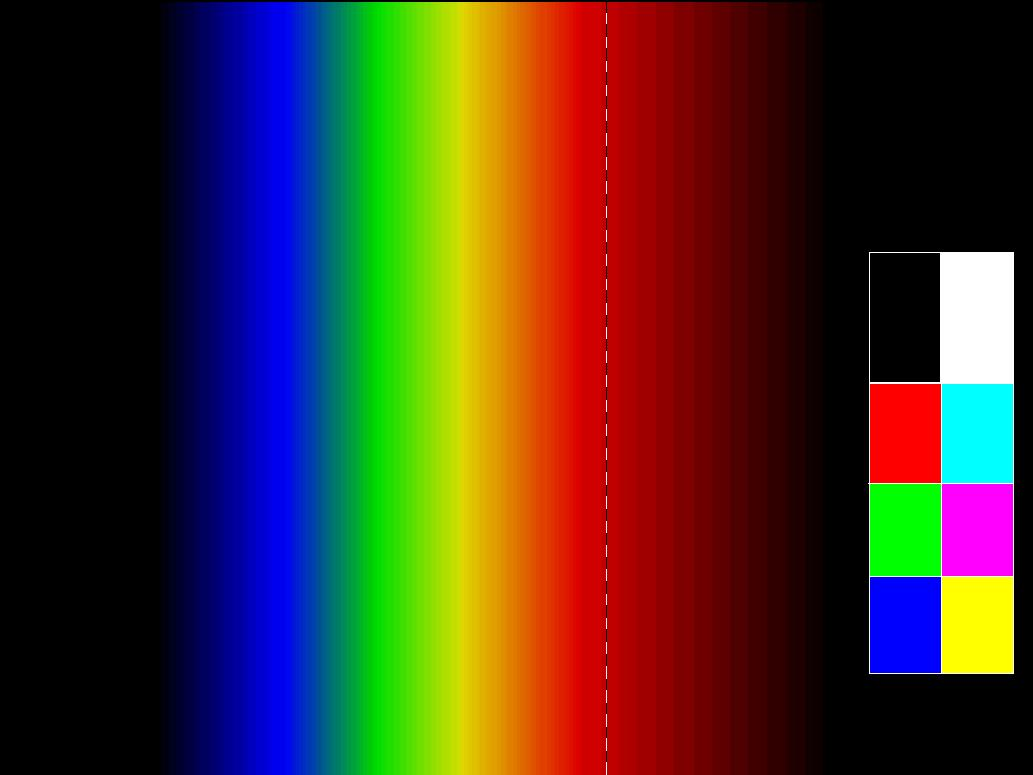
\includegraphics[width=\textwidth]{Graphics/opencvEtalon.jpg}
					        \caption{Spectre de la lumière visible \textit{\textbf{(source : http://physique-eea.ujf-grenoble.fr/)}}}
					    \end{subfigure}\\

					    \begin{subfigure}[h]{0.3\textwidth}
					        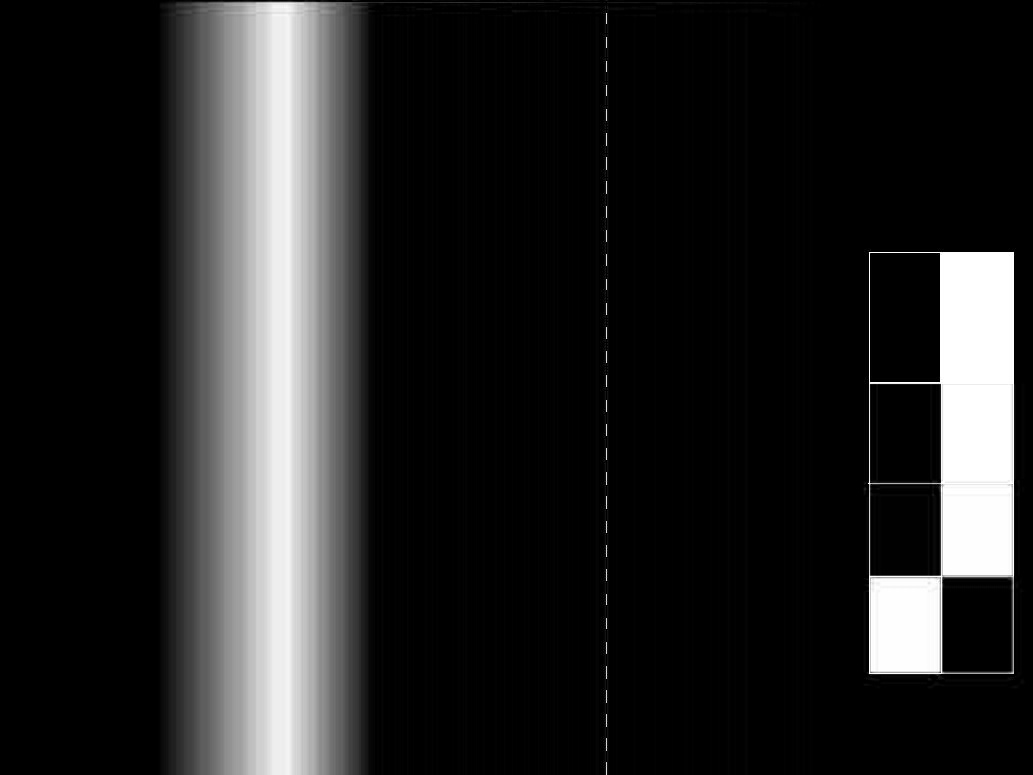
\includegraphics[width=\textwidth]{Graphics/opencvB.jpg}
					        \caption{Filtre bleu}
					    \end{subfigure}
					    ~ %add desired spacing between images, e. g. ~, \quad, \qquad, \hfill etc. 
					      %(or a blank line to force the subfigure onto a new line)
					    \begin{subfigure}[h]{0.3\textwidth}
					        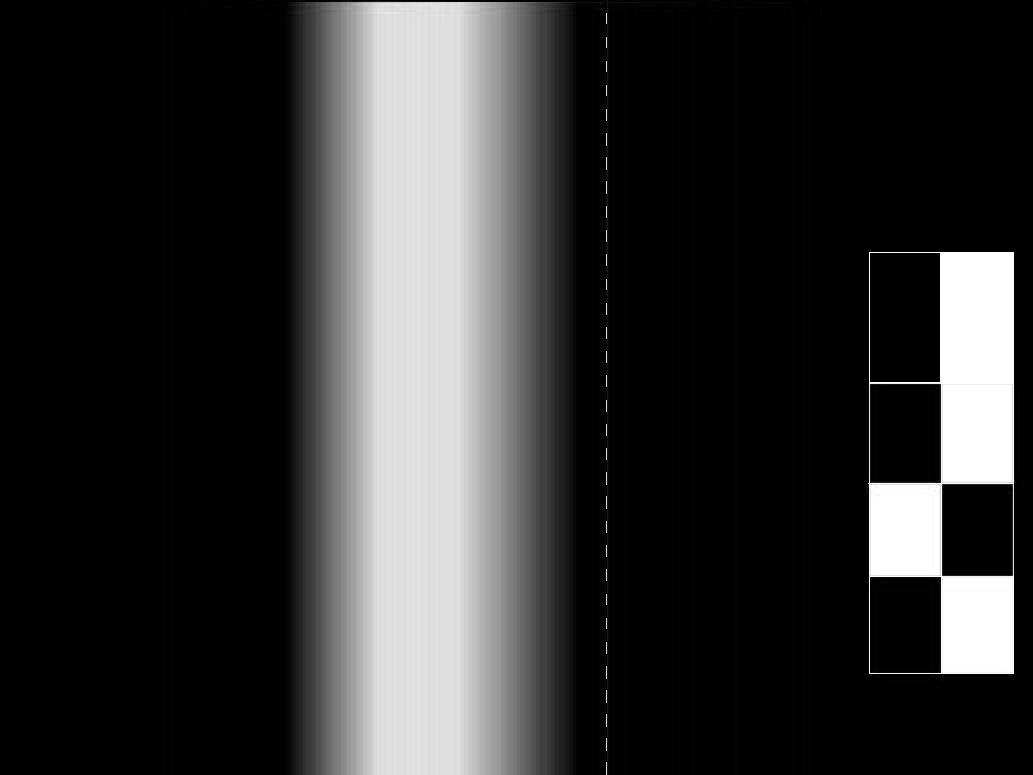
\includegraphics[width=\textwidth]{Graphics/opencvG.jpg}
					        \caption{Filtre vert}
					    \end{subfigure}
					    ~ %add desired spacing between images, e. g. ~, \quad, \qquad, \hfill etc. 
					    %(or a blank line to force the subfigure onto a new line)
					    \begin{subfigure}[h]{0.3\textwidth}
					        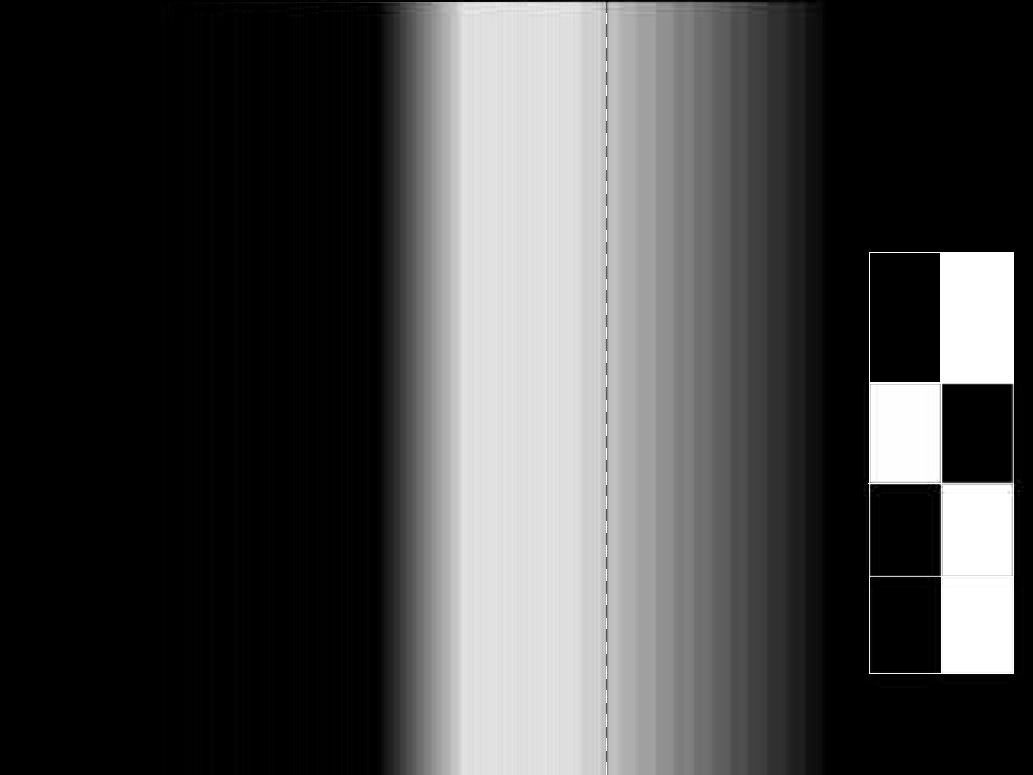
\includegraphics[width=\textwidth]{Graphics/opencvR.jpg}
					        \caption{Filtre rouge}
					    \end{subfigure}

					    \caption{Spectre (a), selon différents filtres (b),(c) et (d).}
					\end{figure}

					Pour des soucis d'optimisations et de résultats, nous n'utiliserons pas le système Rouge-Vert-Bleu classique, mais plutôt le système HSV\label{HSV}\nomenclature{HSV}{Hue-Saturation-Value, ou Teinte-Saturation-Valeur}, plus adapté à notre problématique :

					\begin{figure}[H]
						\centering
						\begin{subfigure}[h]{0.35\textwidth}
					        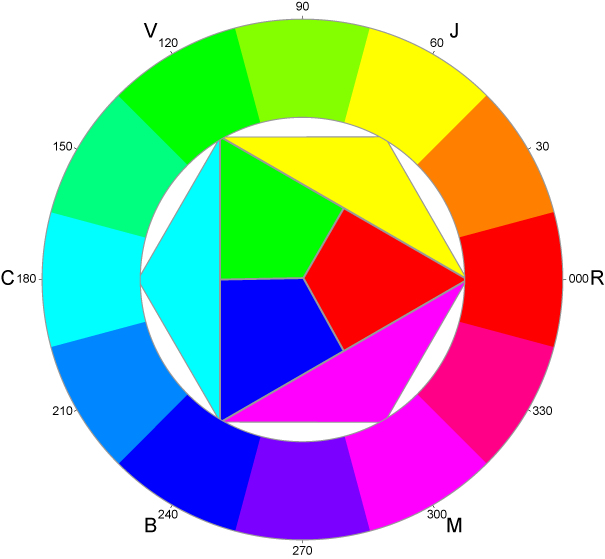
\includegraphics[width=\textwidth]{Graphics/RVB.png}
					        \caption{Modèle RVB}
					    \end{subfigure}
					    ~
					    \begin{subfigure}[h]{0.35\textwidth}
					        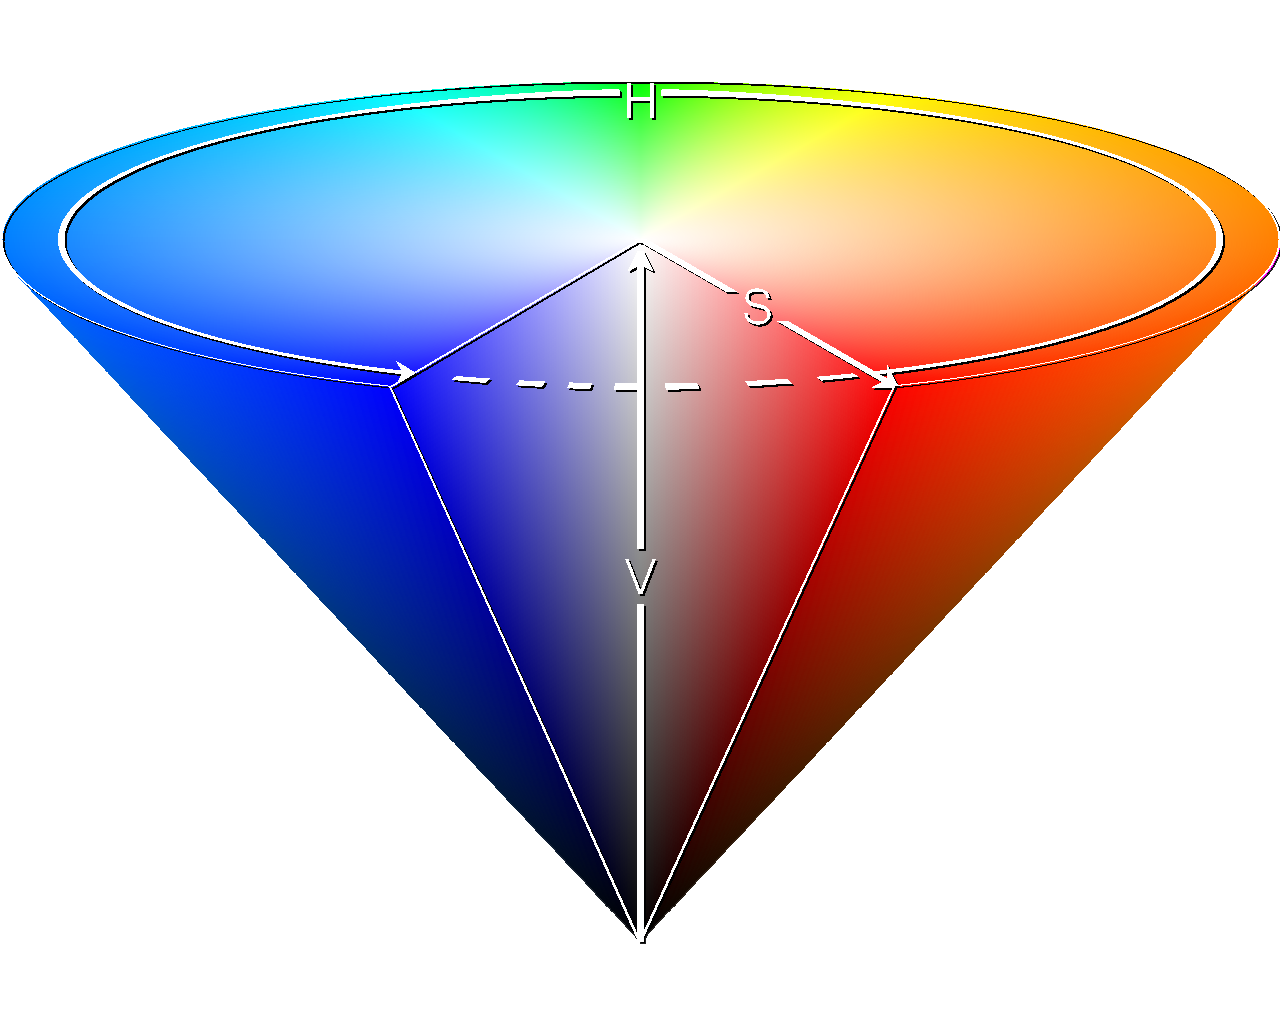
\includegraphics[width=\textwidth]{Graphics/HSV_cone.png}
					        \caption{Modèle HSV}
					    \end{subfigure}
					    \caption{Comparaison RVB / HSV}
					\end{figure}
					Grâce à ce système, il nous suffit de définir expérimentalement les bornes autour de nos 3 axes de couleurs afin de créer un \textit{masque}. Un masque est ici une image (une matrice, un tableau à deux dimensions); chaque case contenant "1" ou "0". Si "0", le pixel n'a pas passé le filtre : il ne nous intéresse pas. En revanche, si "1", ce pixel et ses environs sont potentiellement interessants et devront être analysés. Nous y reviendrons.\\
					La fonction \textit{inRange} est prévue à cet effet, et nous permet de réaliser un tel masque : 
					Nous déterminerons expérimentalement des bornes pour les variables Teinte ($H_{min}$ et $H_{max}$), Saturation ($S_{min}$ et $S_{max}$) et Valeur ($V_{min}$ et $V_{max}$). Soit un pixel $p$ positionné en $i$ avec pour composantes $H_{i,p}$,$S_{i,p}$,$V_{i,p}$, nous aurons la relation suivante :
					\\ 
					$D_i = H_{min} \leqslant H_{i,p} \leqslant H_{max} 	\land S_{min} \leqslant S_{i,p} \leqslant S_{max} \land V_{min} \leqslant V_{i,p} \leqslant V_{max}$ \cite{bib20}
					\\
					Avec $D_i$ valant VRAI ou FAUX. Si $D_i$ est FAUX, cela signifie qu'il n'y a aucune corrélation entre la couleur détectée et notre objet. En revanche, s'il est VRAI, alors notre objet existe PROBABLEMENT dans notre champs de vision. Nous définirons donc expérimentalement deux couples de triplets (correspondant aux bornes pour le feu vert et le feu rouge). De plus, en utilisant les fonctions d'érosion (\textit{erode}) et de dilatation (\textit{dilate}), nous suprimons les pixels parasites qui passeraient le premier filtre, gardant ainsi uniquement le feu.
					\\

					Une autre problématique est la distance à laquelle le robot doit s'arrêter. En effet, si le feu est rouge, il ne faut pas qu'il s'arrête juste à côté de celui-ci : il risquerait de ne pas le voir passer au vert et de rester bloqué. Compte tenu des vitesses engagées et de l'inertie des moteurs et du robot, nous négligerons la distance de freinage.
					Le schéma suivant résume la situation :
					\illu{distEval.pdf}{Schéma de principe de l'approche d'un feu}{0.35}
					Connaissant l'angle de vue de la caméra (58°)\cite{bib18}, et en utilisant des fonctions géométriques simples, nous pouvons déterminer rapidement la distance minimale au feu s'il faut s'arrêter : $d_{min} = 15 cm \times tan(\frac{58}{2}) = 8,3 cm$. En ajoutant une distance de sécurité puisque la distance de freinage est négligée, nous pouvons ainsi déterminer le moment à partir duquel le robot passera le feu quoi qu'il arrive. Cette distance est établie arbitrairement à 10 cm.\\

				\item \textbf{Présence et intentions des autres utilisateurs}

					Les feux sont les plus simples à gérer. En effet, il ne peut y avoir qu'une et une seule position pour un unique feu. Il suffit "juste" de détecter si oui ou non la couleur dans l'intervalle sélectionné existe. Détecter les intentions d'un autre robot est autrement plus difficile. En effet, compte tenu de la disposition des différents clignotants, nous voyons quoi qu'il arrive 3 des 4 clignotants du robot, s'il ne va pas dans le même sens que nous. \\
					Un bon exemple d'un aperçu de la vue du robot est donné par la figure \ref{robotVueExemple}, page \pageref{robotVueExemple}.
					Après filtrage d'après la méthode indiquée ci-dessus, il faudra récupérer sur le masque de l'image obtenu les différentes tâches en utilisant une méthode \textit{itérative} appelée MeanShift ("Déplacement de moyenne"). Le principe est simple : on choisit un point de coordonnées $(x_0,y_0)$. Autour de ce point, on définit une zone correspondant à la zone d'étude de rayon $r$. On calcule donc la moyenne des coordonnées de chaque "1" du masque contenu dans la zone d'étude. Si aucun n'est contenu dans l'intervalle $[x_0 - r \leqslant x \leqslant x_0 + r ; y_0 - r \leqslant y \leqslant y_0 + r ]$, on décale le point en dehors de ce rayon. Sinon, calcule la moyenne des coordonnées des points compris dans cet intervalle. On obtient ainsi un nouveau point coordonnées $(x_1,y_1)$. L'opération est \textit{réitérée} autant de fois que nécessaire pour déterminer la position d'une LED. Cet algorithme permet de \textit{converger} vers la plus grande densité de points du masque : la LED. Le schéma suivant illustre le fonctionnement de cette méthode.
					\illu{meanShiftMethode.pdf}{Principe de fonctionnement de la méthode "MeanShift" à 3 itérations}{1.2}
					Le même procédé est appliqué une seconde fois. L'algorithme veut qu'un point "cherchant une LED" ne rentre pas dans la zone d'étude d'un autre point ayant déjà localisé une LED, afin de ne pas créer de doublon pouvant fausser les résultats. Si cette deuxième recherche de led est infructeuse, cela signifie que l'on se situe dans un des deux cas suivants :

					\begin{figure}[H]
						\centering
						\begin{subfigure}[h]{0.2\textwidth}
					        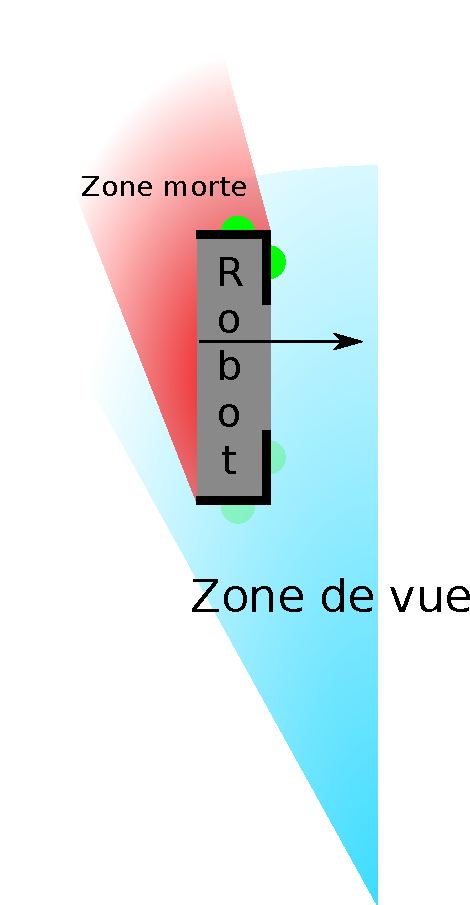
\includegraphics[width=\textwidth]{Graphics/casClignotants_DG.pdf}
					        \caption{Robot à gauche tournant à gauche}
					    \end{subfigure}
					    ~
						\begin{subfigure}[h]{0.35\textwidth}
					        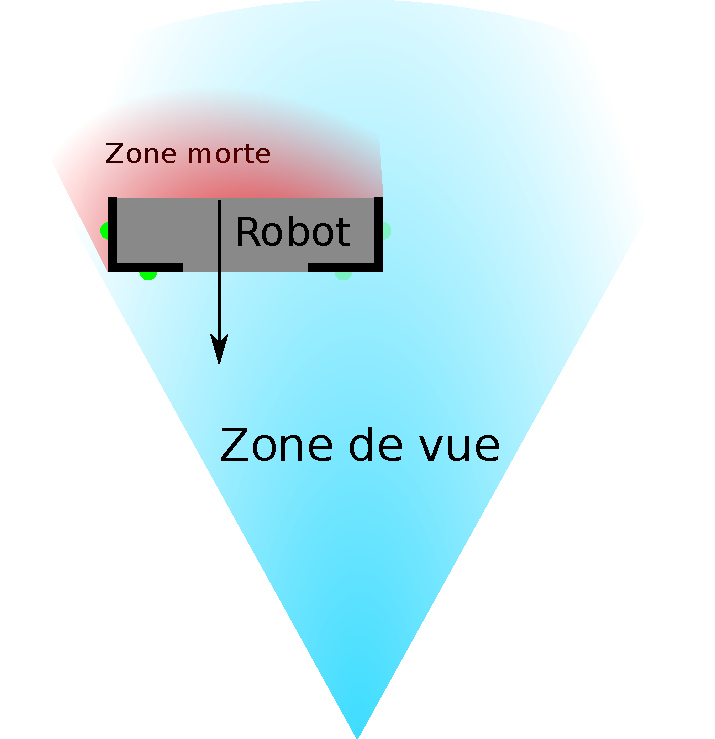
\includegraphics[width=\textwidth]{Graphics/casClignotants_AD.pdf}
					        \caption{Robot devant tournant à droite}
					    \end{subfigure}
					    ~
					    \begin{subfigure}[h]{0.2\textwidth}
					        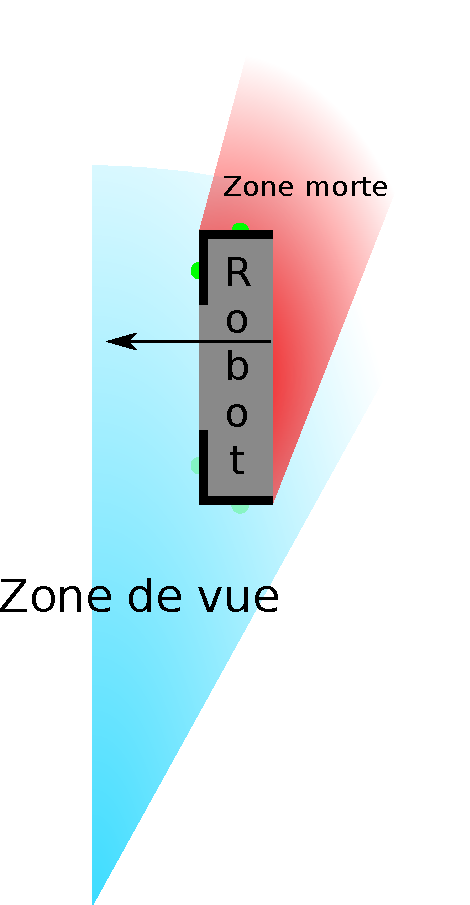
\includegraphics[width=\textwidth]{Graphics/casClignotants_GD.pdf}
					        \caption{Robot à droite tournant à droite}
					    \end{subfigure}
					    \caption{Cas d'une seule LED détectée}
					\end{figure}
					Si une situation comme cela apparait, on repère la position abolue de la LED. Si celle-ci se trouve sur la moitié droite du masque, cela signifie que l'on se situe dans le cas (c). Si la LED se situe sur le bord gauche, deux possibilités s'offrent à nous : soit on se trouve dans la situation (b), auquel cas on se situera au carrefour. Si notre feu est vert et que l'on décide de tourner à gauche également, il faudra combiner ces données au sonar. Si on décide d'aller tout droit ou à droite, on pourra traverser le carrefour sans soucis. En revanche, si on se trouve dans la situation (a), on a à nouveau deux possibilités : soit on se situe au carrefour central auquel cas un des deux robot sera arrété à cause du feu, donc aucun danger, soit on se trouve à une intersection : la règle de la priorité à droite d'applique, nous pouvons avancer sans être inquiétés.
					\\
					Voici les trois autres cas restants :
					\begin{figure}[H]
						\centering
						\begin{subfigure}[h]{0.2\textwidth}
					        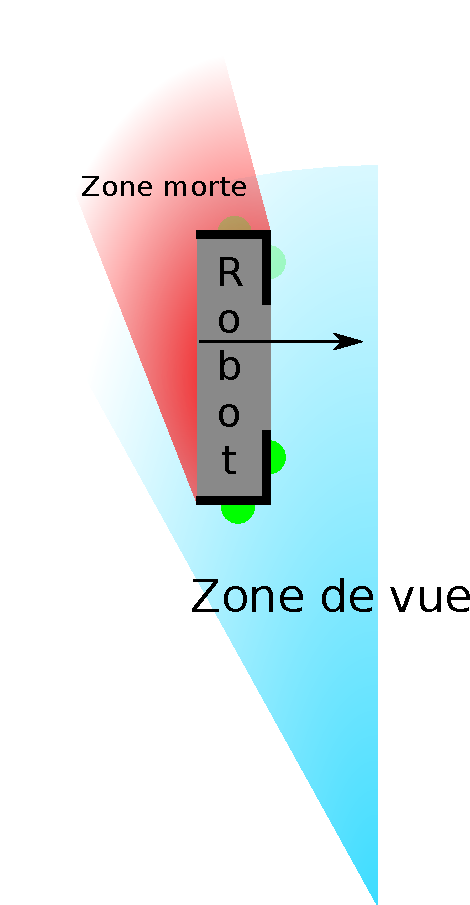
\includegraphics[width=\textwidth]{Graphics/casClignotants_DD.pdf}
					        \caption{Robot devant tournant à gauche}
					    \end{subfigure}
					    ~
						\begin{subfigure}[h]{0.35\textwidth}
					        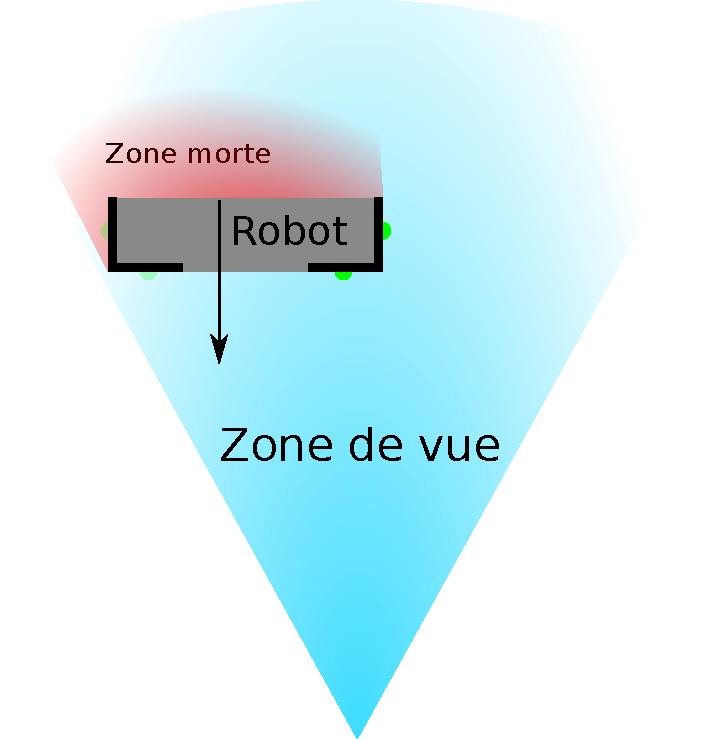
\includegraphics[width=\textwidth]{Graphics/casClignotants_AG.pdf}
					        \caption{Robot devant tournant à gauche}
					    \end{subfigure}
					    ~
					    \begin{subfigure}[h]{0.2\textwidth}
					        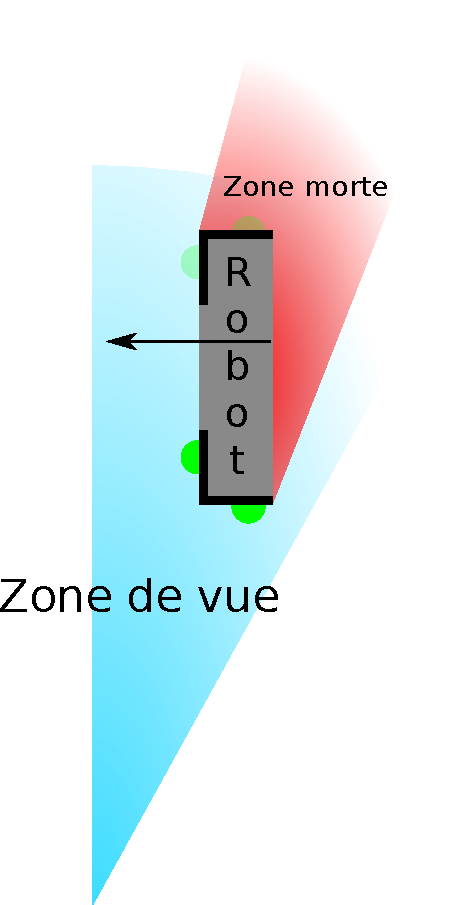
\includegraphics[width=\textwidth]{Graphics/casClignotants_GG.pdf}
					        \caption{Robot à droite tournant à gauche}
					    \end{subfigure}
					    \caption{Cas de deux LEDs détectées}
					\end{figure}

					Une fois encore, on réalise un masque et on repère la position des 2 LEDs. Cette fois, on "découpe" le masque en trois verticalement : si les LEDs sont dans le tier de gauche (a), l'agent est à gauche et désire tourner à droite. Si les LEDs sont dans le tier de droite (c), le robot, situé à droite, souhaitera tourner à gauche, et donc croiser notre trajectoire. Il s'agira là de faire respecter la règle de la priorité à droite. Enfin, si celles-ci sont dans le tier du milieu (b), cela signifie que le robot est en face et désire tourner à gauche, et croiser notre trajectoire.
					\\
					On démontre ainsi ici qu'avec une simple asymétrie, on arrive facilement à prédire le comportement des autres usagers.
					\\
					D'un point de vue plus généraliste, si nous considérons une voiture autonome, la détection visuelle des intentions des utilisateurs alentours est une étape à considérer pendant la phase de transition correspondant à l'apparition des voitures autonomes sur le réseau urbain.
			\end{itemize}